\documentclass[conference]{IEEEtran}

\usepackage{cite}

\usepackage[cmex10]{amsmath}

\usepackage[pdftex]{graphicx}

\usepackage{tabularx}


\usepackage{algorithm}
\usepackage[noend]{algpseudocode}

\usepackage[tight,footnotesize]{subfigure}



\begin{document}


\newtheorem{definition}{\textbf{Definition}}
\newtheorem{lemma}{\textbf{Lemma}}
\newtheorem{theorem}{\textbf{Theorem}}
\newtheorem{claim}{\textbf{Claim}}
\newtheorem{corollary}{\textbf{Corollary}}
\newtheorem{observation}{\textbf{Observation}}
\newtheorem{property}{\textbf{Property}}



\title{How to write papers using LaTex}

\author{\IEEEauthorblockN{
Chick\IEEEauthorrefmark{1},
Duck\IEEEauthorrefmark{2}}
\IEEEauthorblockA{\IEEEauthorrefmark{1}State Key Laboratory for Novel Software Technology, Nanjing University, Nanjing 210024, China}
\IEEEauthorblockA{\IEEEauthorrefmark{2}Department of Computer Science, City University of Hong Kong, Hong Kong}
}

\maketitle

\begin{abstract}
This article describes how to use LaTex to write academic papers. It is written to help absolute beginners to gain a glimpse of how academic paper is organized using LaTex. Technical details and fancy tricks of LaTex will not be covered in this article(as I do not know any of them). Hopefully, this can serve as a template or maybe a reference when some of us set out to write a paper. 
\end{abstract}

% It is common practice to organize your paper into multiple latex files
% Here, we put only abstract in the main.tex

%!TEX root = main.tex
\section{Introduction}
\label{sec:intro}
In Introduction, we introduce the background of our work, describe briefly the problems we discover and the contribution we make.
%!TEX root = main.tex
\section{Related Work}
\label{sec:related}

In this section, we introduce related prior work regarding this paper's research topic. Usually, this section involves lots of citations.
citation works like this: \cite{adams_davies_2009}.
%!TEX root = main.tex
\section{Problem and Statement}
\label{sec:model}

BGMDD(bipartite graph matching with dynamic duration) problem(Sec. \uppercase\expandafter{\romannumeral3}-A)  and important concepts such as regret(Sec. \uppercase\expandafter{\romannumeral3}-B) are defined in this section. Table \uppercase\expandafter{\romannumeral1} lists the notation and basic definitions.

\subsection{Problem Definition}

\begin{definition}
(Dynamic Bipartite Graph, DBG). \emph{A dynamic bipartite graph is defined as $B=(L,R,E)$, where $L=\{i \in \mathbb{N}\}$ and  $R={j \in \mathbb{N}}$ are  the sets of left and right nodes and $E\in L\times R$ is the set of edges between $L$ and $R$. The node in $L$ or $R$ arrives independently from known probability distributions $P_{L}=\{p_l\}$ or $P_{R}=\{p_r\}$. Each node $i(j)$ arrives at time i(j), which is meaning to abuse the index to denote the nodes' arriving time. Each node has duration denoted by $i.d(j.d)$. If a node is not matched during the duration, the node would leave. Each edge $(i,j)\in E$ has a weight denoted by $e_ij$ obeyed a distribution $P_E=\{p_e\}$.}
\end{definition}
\begin{definition}
(Matching Allocation). \emph{A matching allocation over a dynamic bipartite graph B is denoted by $M =\{(i, j)|i \in L, j \in R\}$. It is a set of node pairs where each node appears at most once.The utility score of a matching allocation $M$ over a dynamic bipartite graph $B$ is measured by $U(B, M) = \{(i,j)\in M w(i, j)\}$.}
\end{definition}

\par In a real word, the nodes arriving distributions ($P_{L}=\{p_l\}$  $P_{R}=\{p_r\}$ ) and the edge weight distribution($P_E=\{p_e\}$) may change after some time. But it's easy to confirm the changes by collecting statistics. So in order to analysis convenient, we assume the distributions($P_{L}=\{p_l\}$, $P_{R}=\{p_r\}$ and $P_E=\{p_e\}$) are permanent. Alough by collecting statistics some changes could be measured, the change of duration of nodes can not be measured unless we doesn't match nodes and wait until the nodes leaving. It's impossible to do that to measure the changed of the duration. 

\begin{definition}
(Dynamic Duration Distribution.) \emph{Each node's duration obey a distribution $P_ld$(or $P_rd$) independently. In this paper, we first analyze the situation that the durations of nodes in  $L$ and $R$ obey the same distribution $P_d$, $P_d=P_ld= P_rd$. $P_d$ can change after some time unknown.  And we assume the type of the distribution should be pernament. The change of $P_d$ is the decrease or increase of expectation of distribution.  The length of the time in which $P_d$ is stable should not be short. }
\end{definition}
\par The change of duration distribution could be observed in many application scenarios. For example, in the food felivered scene, the customers' patient (which could be considered as duration) are always good in the early time,like 10:30 am (people are not very hungry), but very bad in1:30 am. The same situation would exist in online taxi-hailing service.
\begin{example}
xxxxxxxx
\end{example}
\begin{definition}
(BGMDD problem). \emph{Give a dynamic bipartite graph with duration changed dynamic, the BGMDD problem is to find a matching allcation $M$ to maximize the utility score in the online scenario. }
\end{definition}
\par The BGMDD problem inherits and develops the two-sided online maximum bipartite matching problem in which the duration is  given upon nodes' arrival. And it's also different from ......xxxx

\subsection{MDP and Bandit Modeling for BGMDD problem}
\par When the duration distribution is permanent, [X] states that the batch splitting way to solve DBG problem (dynamic bipartite graph) is a \emph{Markov decision process (MDP)}. The current sets of  left and right nodes and edges can be considered as state space, $\mathcal{S}$. The way to match the nodes, include matching or not matching and how to match, could be considered as action space, $\mathcal{A}$. Obviously, when $P_R$, $P_L$, $P_e$ and $P_d$ are pernament, the transition distribution, $T_r:(\mathcal{S} \times \mathcal{A} \times \mathcal{S})$, is deterministic. The  utility score of matching is the reward, $R_w:(\mathcal{S} \times \mathcal{A}\rightarrow \mathbb{R})$. The target is to maxmine the cumulative score.
\par But when the duration distribution is dynamic, the analyzation should be changed. Because when $P_d$ is dynamic, the the transition distibution is dynamic too. The process should not be considered as standard \emph{MDP}. Instead, the total process can be considered as the combination of bandit problem and  \emph{standard MDP}. We can find that process during the stable time of $P_d$ is \emph{standard MDP} . So the problem translates into \emph{multi-MDPs}. If we can measure the change of $P_d$, we just need to switch solving strategy to the corresponding \emph{MDP}. 
\par But as mention above, the changed of $P_d$ can not be measured directly. So the problem becomes a bandit problem. We can use a ``strategy'' to decide how to match, and after a round(include hundreds of time interval) we need to calculate the total ``reward''(cumulative score) and decide which strategy should be used for next round according to the history. So the strategys corresponding to different \emph{standard MDPs} are considered as ``arms'' in bandit literature. The ``bandit'' property of  BGMDD problem would be proved in section$xx$.
\par In conclusion, the process of BGMDD problem is \emph{MDP} from micro aspect and a ``bandit problem'' in macro angle.

\subsection{Evaluation Metric}
\subsubsection{Competitive Ratio}
xxx
\subsubsection{Regret}
xxx

\subsection{Greedy Algorithm}
\par If we don't care about the total score or competitive ratio, almost all dynamic bipartite graph problem could be solved by Greedy algorithm. Greedy algorithm matches the nodes with the maximum edge weight, and don't match when no nodes can be matched. 
\par  Greedy algorithm don't use the duration actively, for it always matches nodes as soon as possible. So compared to other algorithms which use duration to wait for the better match,  Greedy algorithm can't get the better result. But as compensation, Greedy algorithm is so stablely that the  number of  ``losing node'' which mean the nodes isn't matched during the their duration and leave may be less.
\par It seems that the score of Greedy algorithm is unrelated to duration. However their relevance are very strong. We would prove that there is a positive correlation between the score of Greedy algorithm and the duration(Section xxx).


\begin{property}
Kittens are cute.
\end{property}

\begin{lemma}
People love cute things.
\end{lemma}


\begin{IEEEproof}
Trivial.
\end{IEEEproof}


\begin{subequations}\label{opt:mcup}

\end{subequations}

%!TEX root = main.tex
\section{Algorithm}
\label{sec:alg}

\begin{algorithm}[H]
\caption{Put your caption here}
\begin{algorithmic}[1]

\Procedure{proc}{$a,b$}       \Comment{This is an example}
    \State System Initialization
    \State Read the value 
    \If{$condition = True$}
        \State Do this
        \If{$Condition \geq 1$}
        \State Do that
        \ElsIf{$Condition \neq 5$}
        \State Do another
        \State Do that as well
        \Else
        \State Do otherwise
        \EndIf
    \EndIf

    \While{$something \not= 0$}  \Comment{put some comments here}
        \State $var1 \leftarrow var2$  \Comment{another comment}
        \State $var3 \leftarrow var4$
    \EndWhile  \label{roy's loop}
\EndProcedure
\end{algorithmic}
\end{algorithm}



%!TEX root = main.tex
\section{evaluation}
\label{sec:eva}

Since evaluation section is where figures and tables appear the most, I put examples of inserting figures and tables here, but they can be used elsewhere.

\subsection{figures}

\begin{figure}[H]
\centering
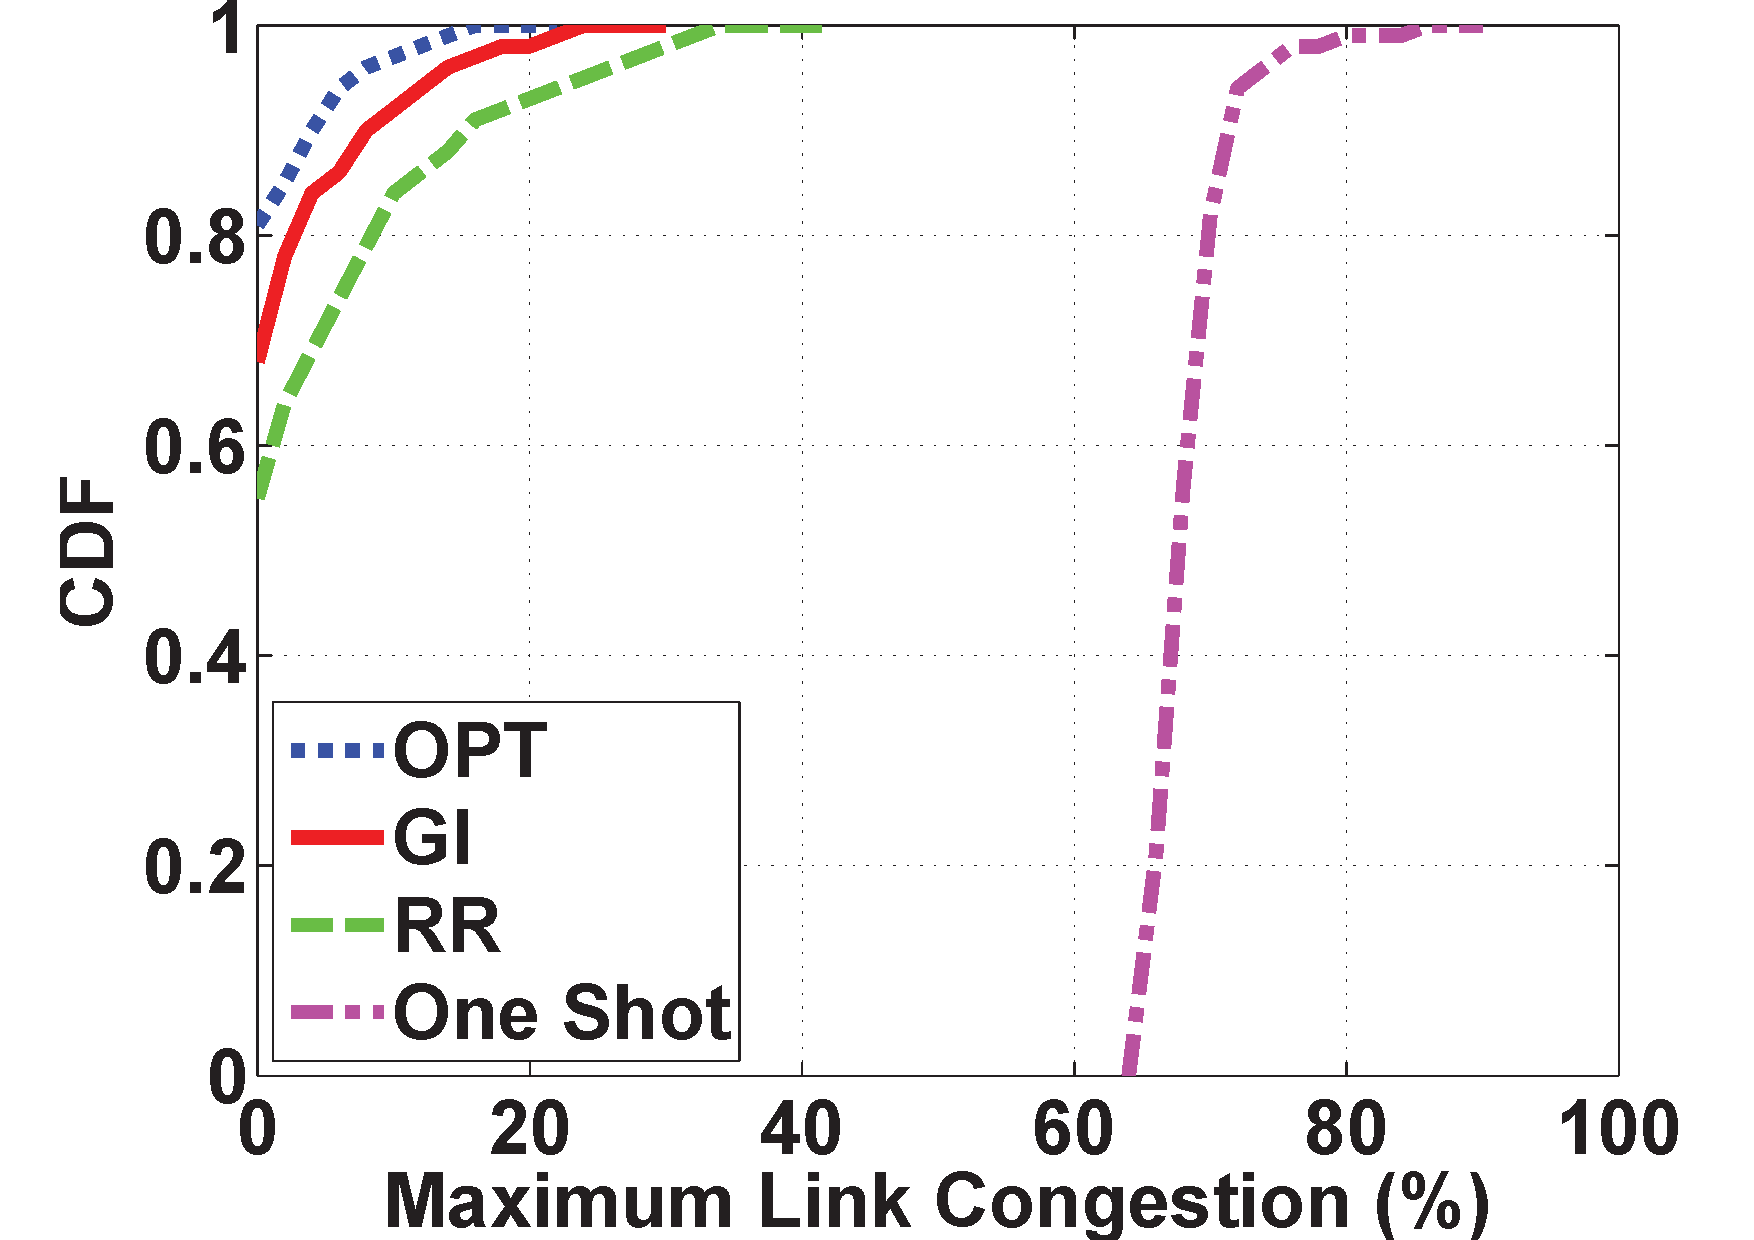
\includegraphics[width=2.0in]{Fig/DCN.pdf}
\caption{insert one figure}
\label{fig:DCN}
\vspace{-3mm}
\end{figure}

\begin{figure}[H]
\subfigure[fig1]{
\begin{minipage}[b]{0.2\textwidth}
\label{fig:TopologyDCN}
\centering
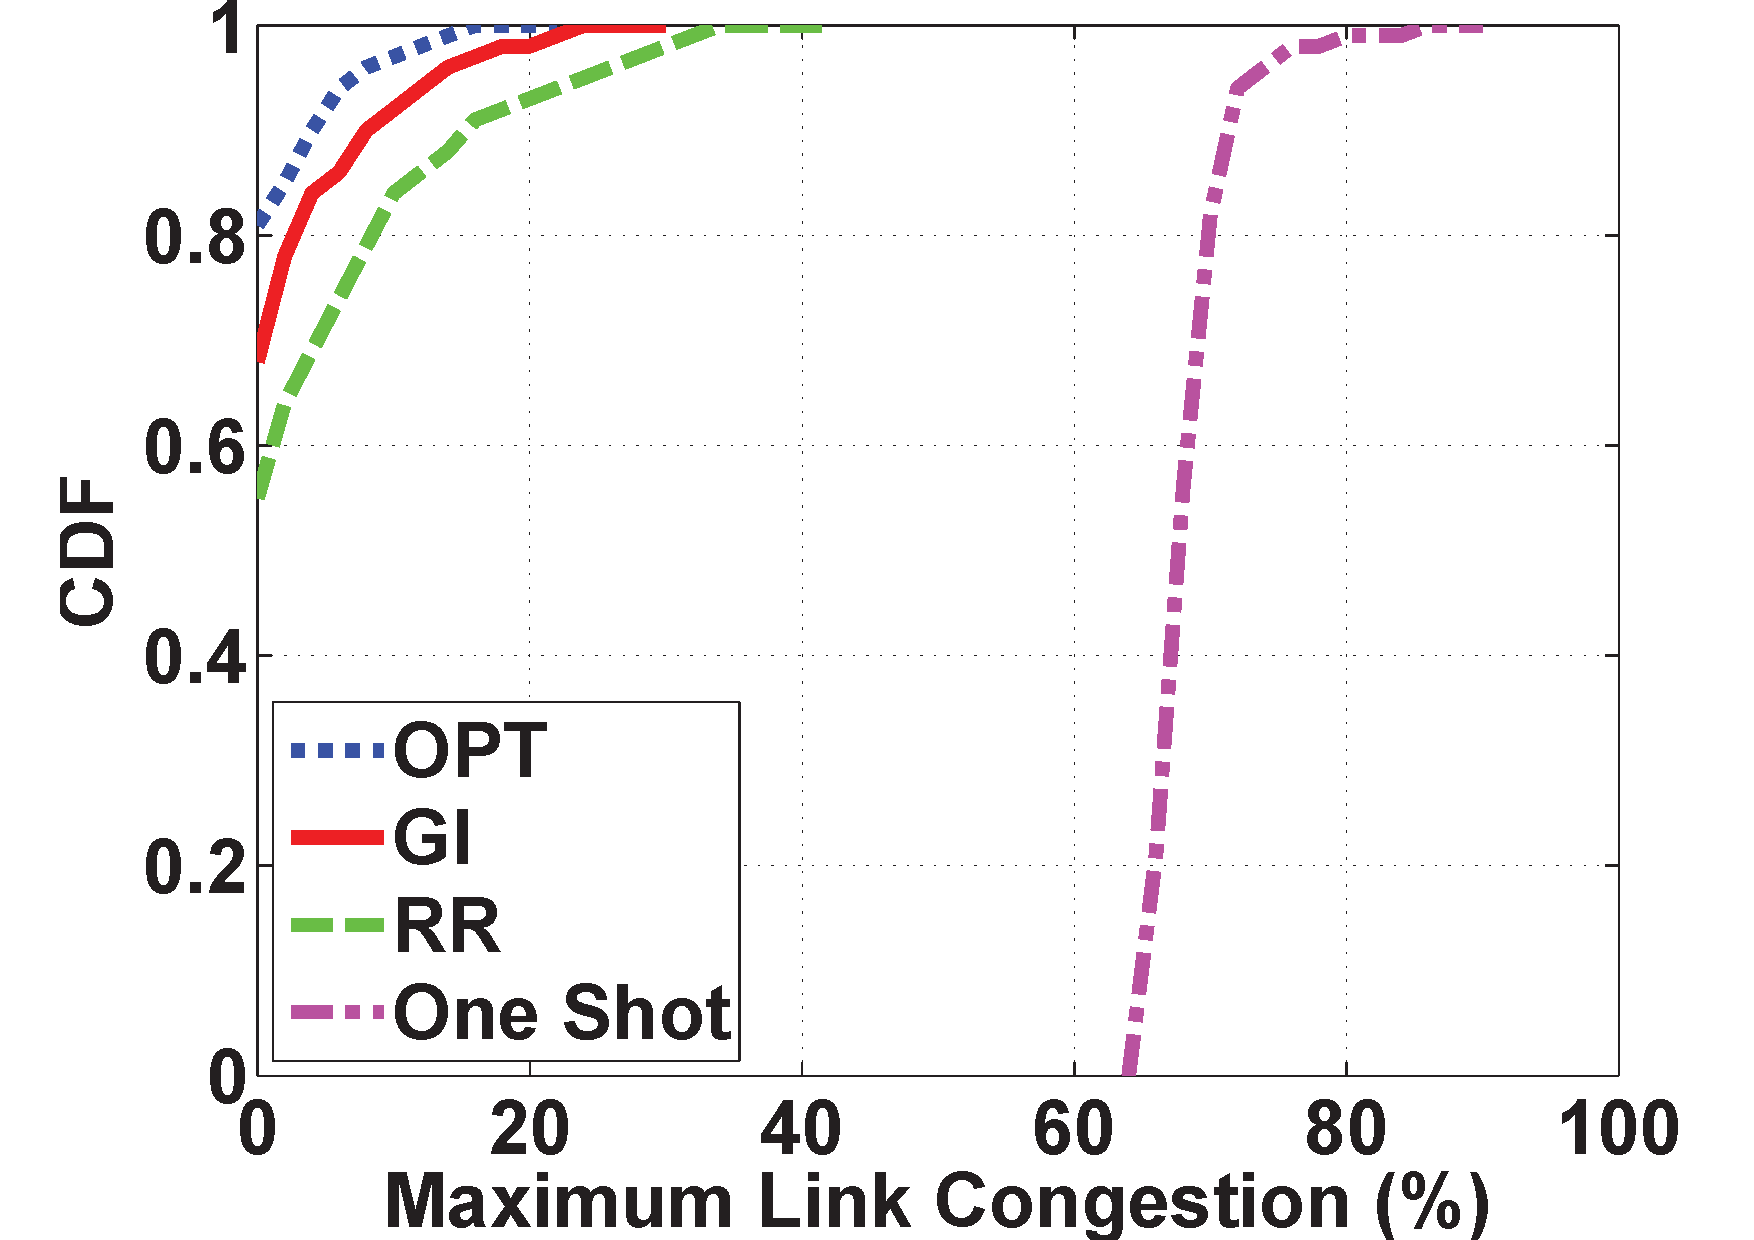
\includegraphics[width=1.5in]{Fig/DCN.pdf}
\end{minipage}}
\subfigure[fig2]{
\begin{minipage}[b]{0.2\textwidth}
\label{fig:TopologyWAN}
\centering
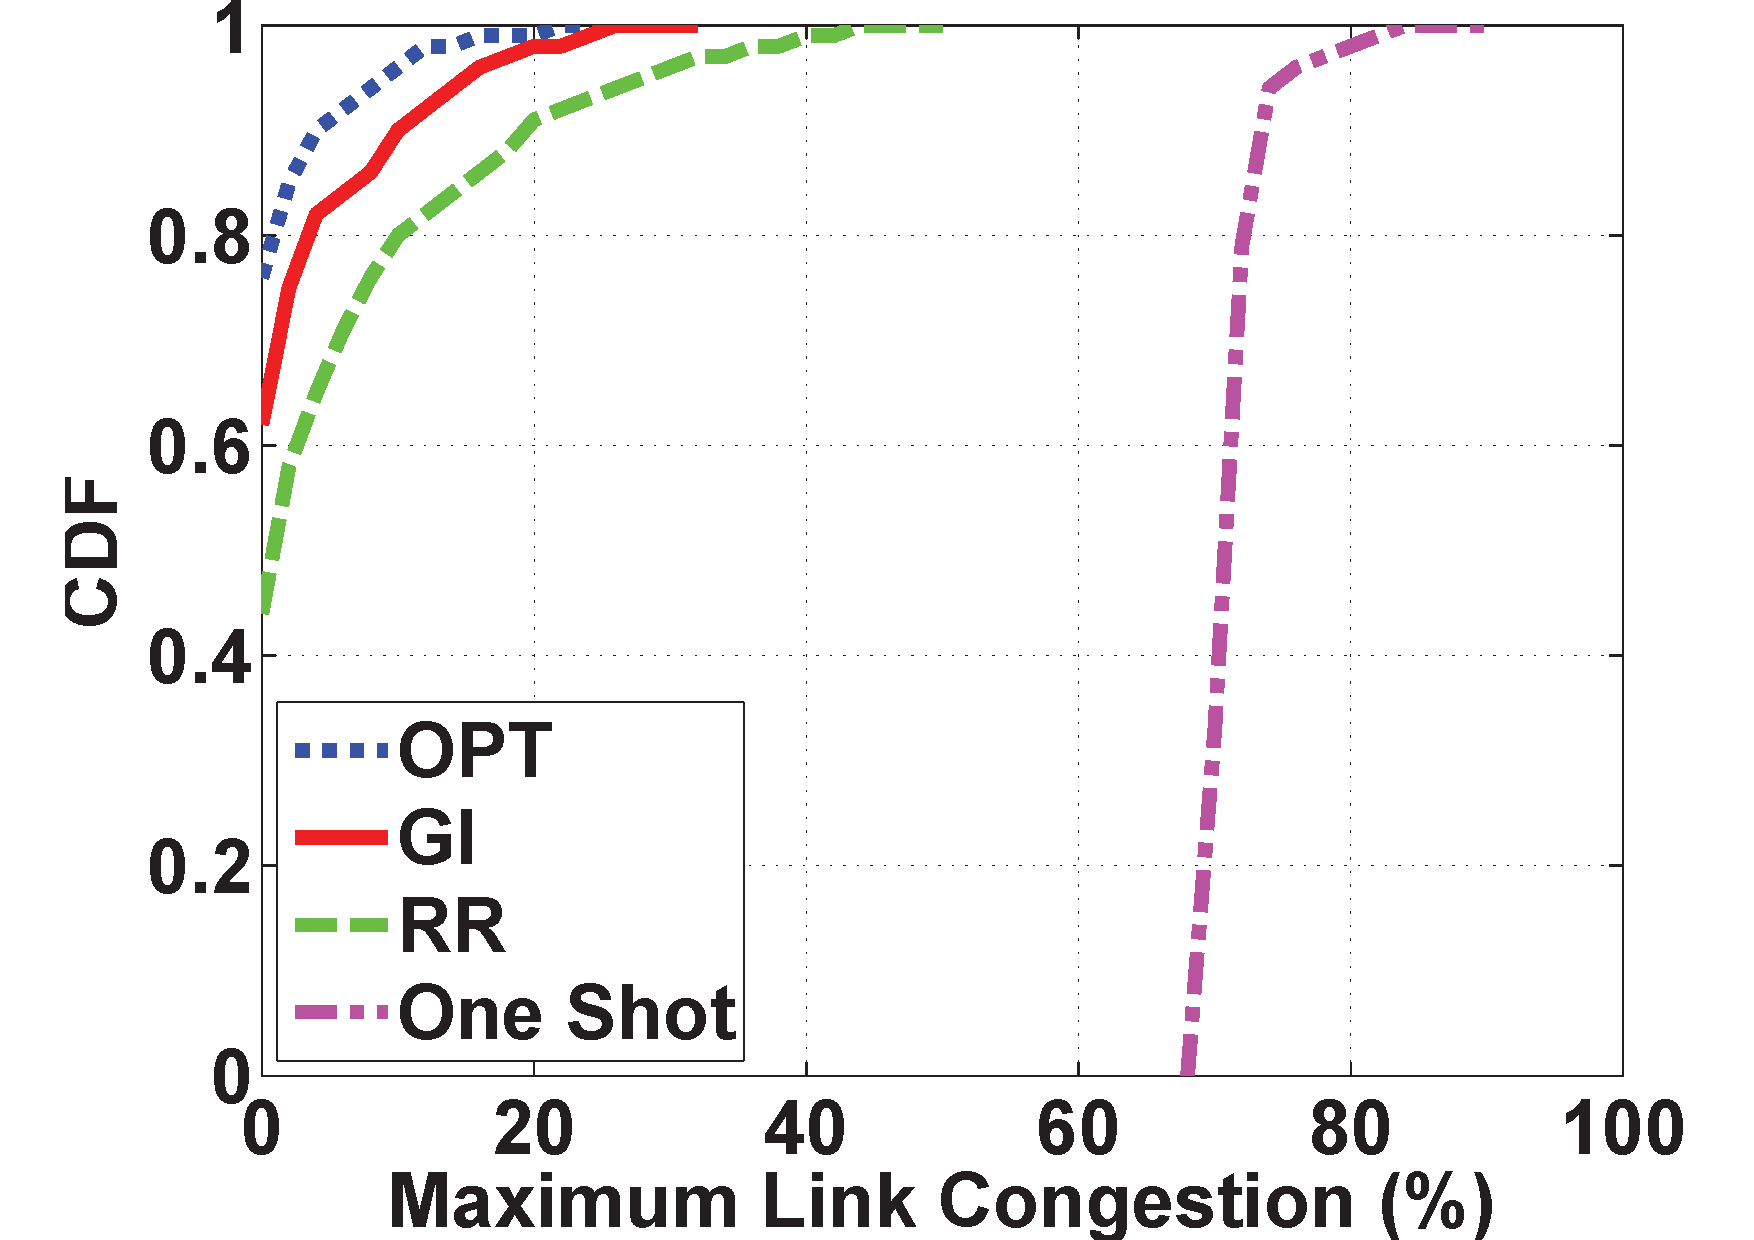
\includegraphics[width=1.5in]{Fig/WAN.pdf}
\end{minipage}}
\caption{put two figures together horizontally} \label{fig:Topology}
\vspace{-1em}
\end{figure}


\begin{figure*}[t]
\begin{minipage}[t]{0.49\textwidth}
\subfigure[DCN scenario]{
\label{fig:DCN}
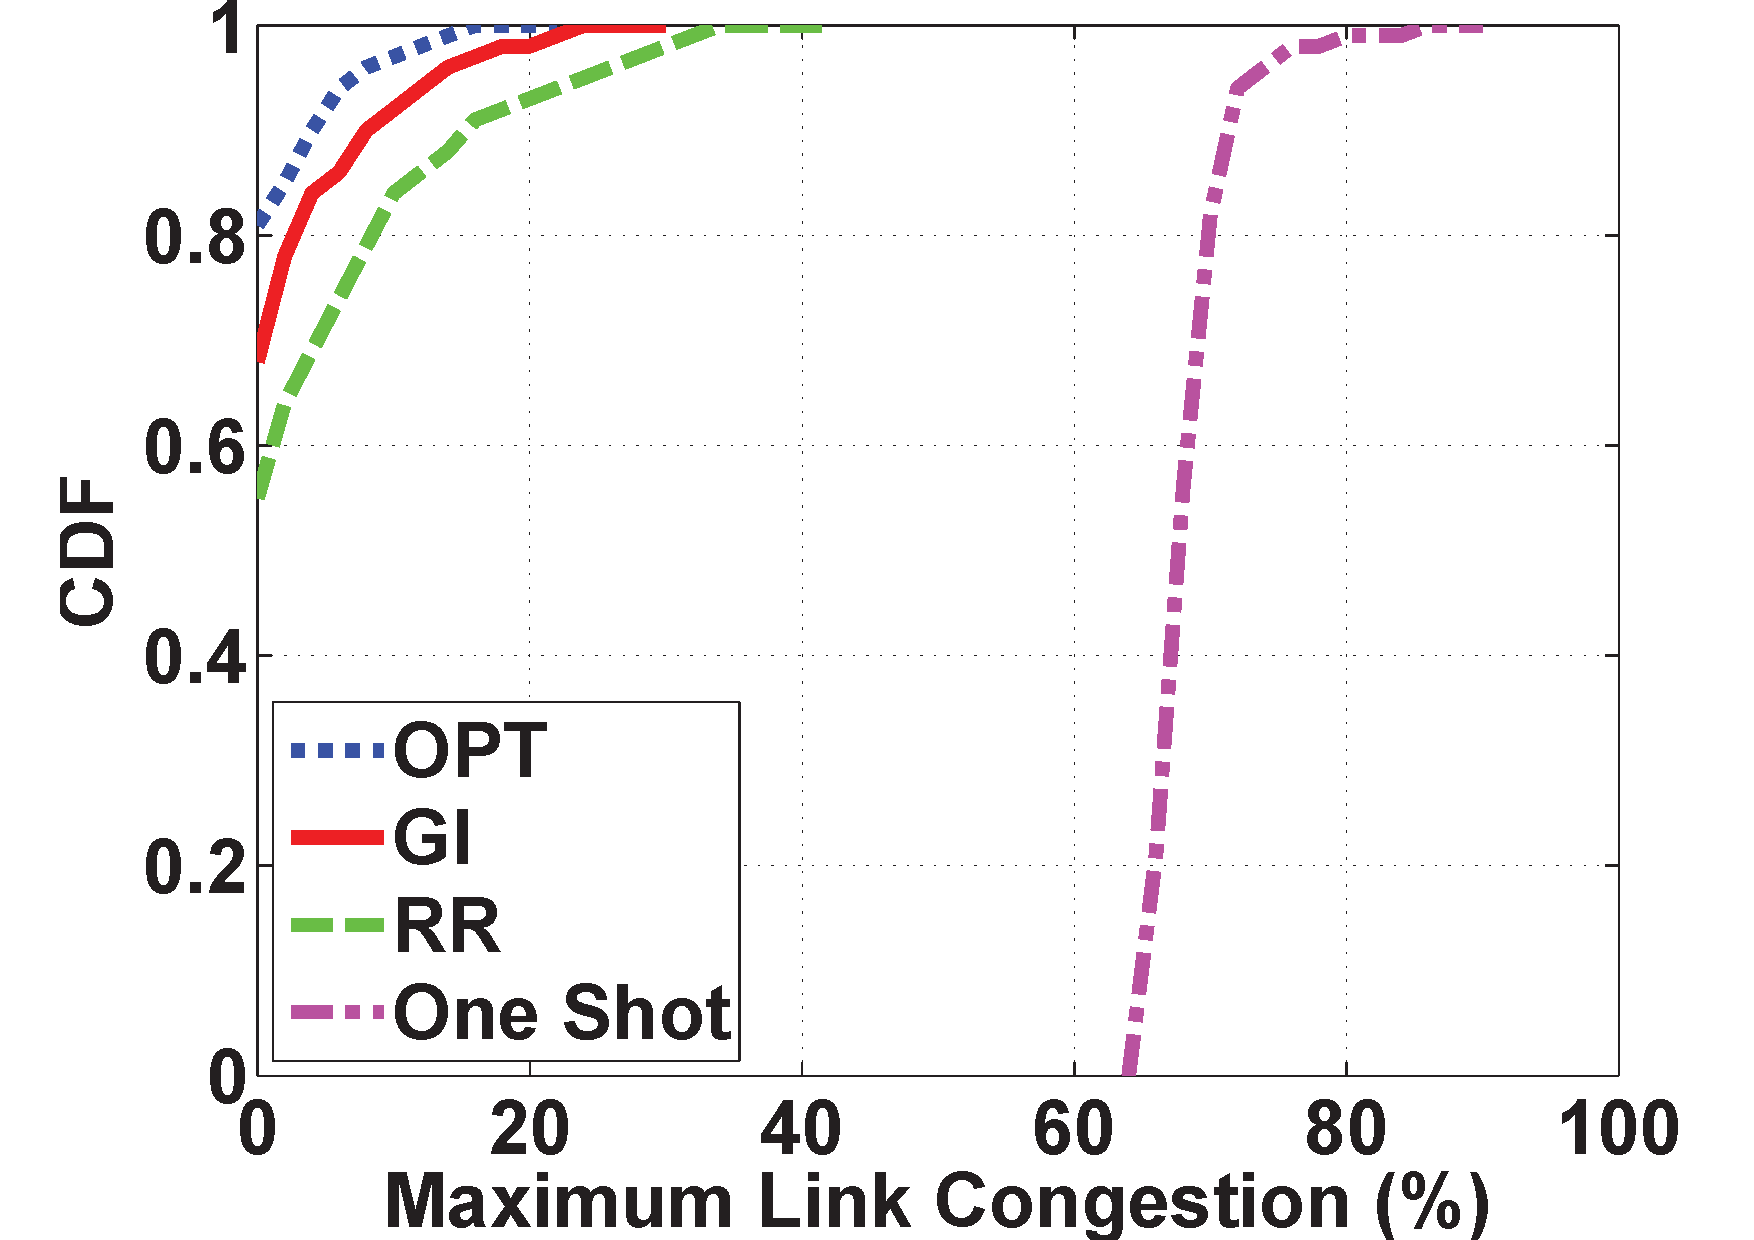
\includegraphics[width=1.6in]{Fig/DCN.pdf}}
\subfigure[WAN scenario]{
\label{fig:WAN}
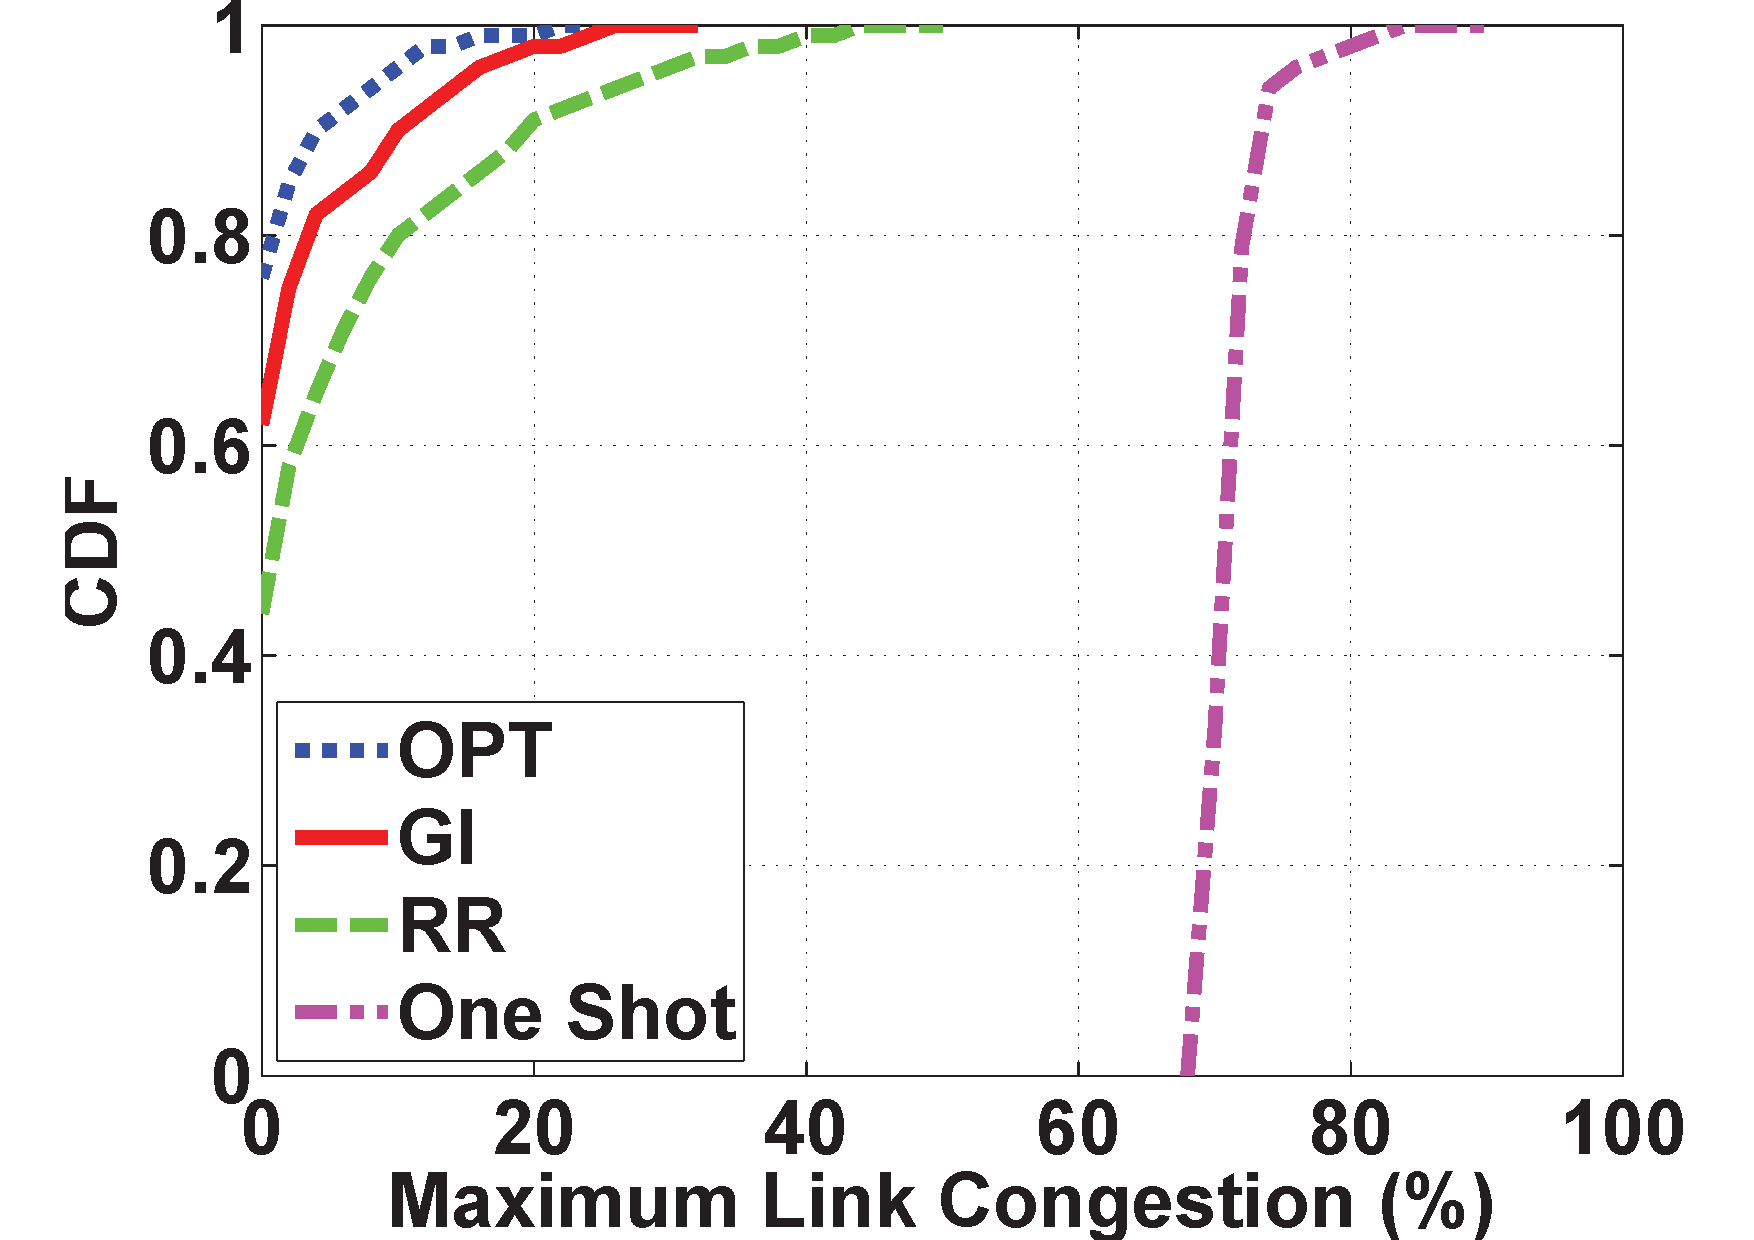
\includegraphics[width=1.6in]{Fig/WAN.pdf}}
\caption{Maximum link congestion comparison.}
\label{fig:LinkCongestion}
\end{minipage}
\begin{minipage}[t]{0.49\textwidth}
\subfigure[DCN scenario]{
\label{fig:RunningTimeDCN}
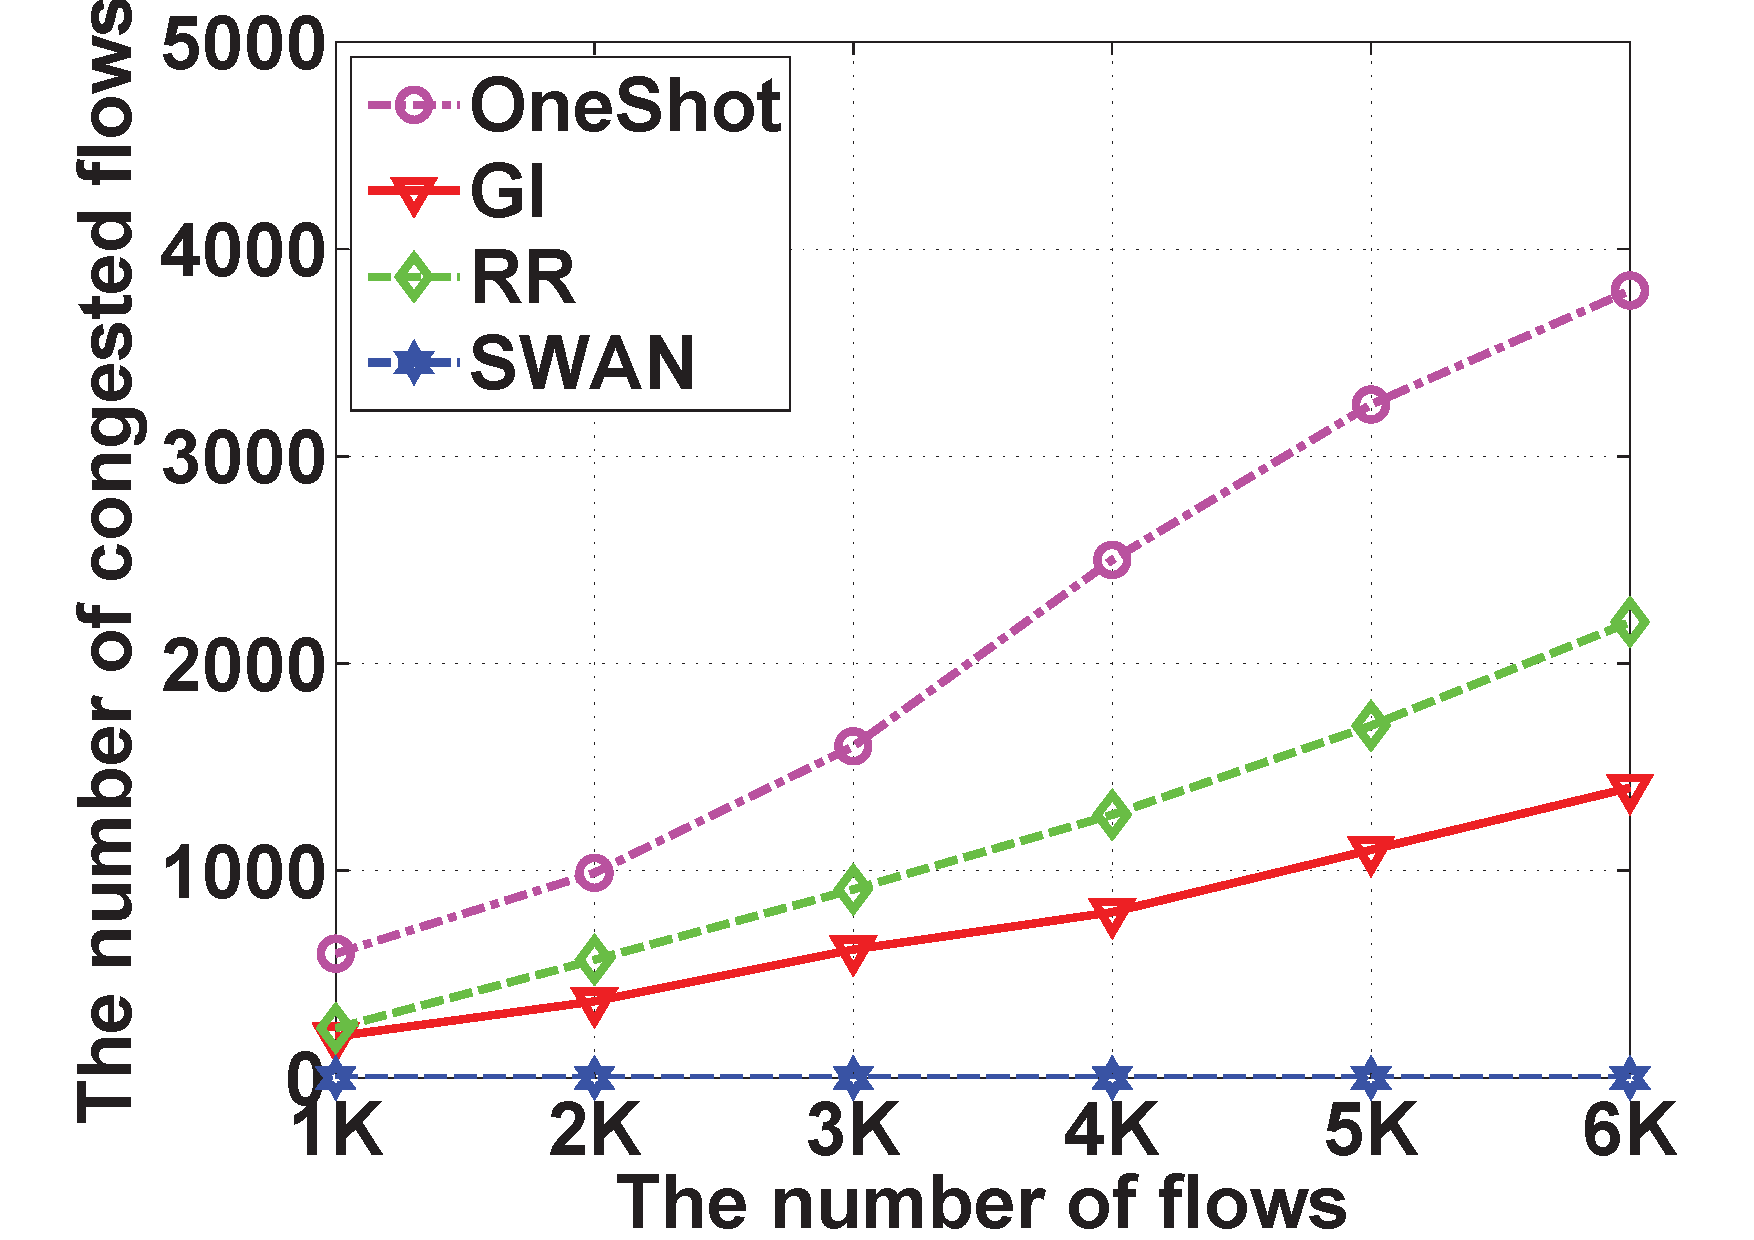
\includegraphics[width=1.6in]{Fig/RTDCN.pdf}}
\subfigure[WAN scenario]{
\label{fig:RunningTimeWAN}
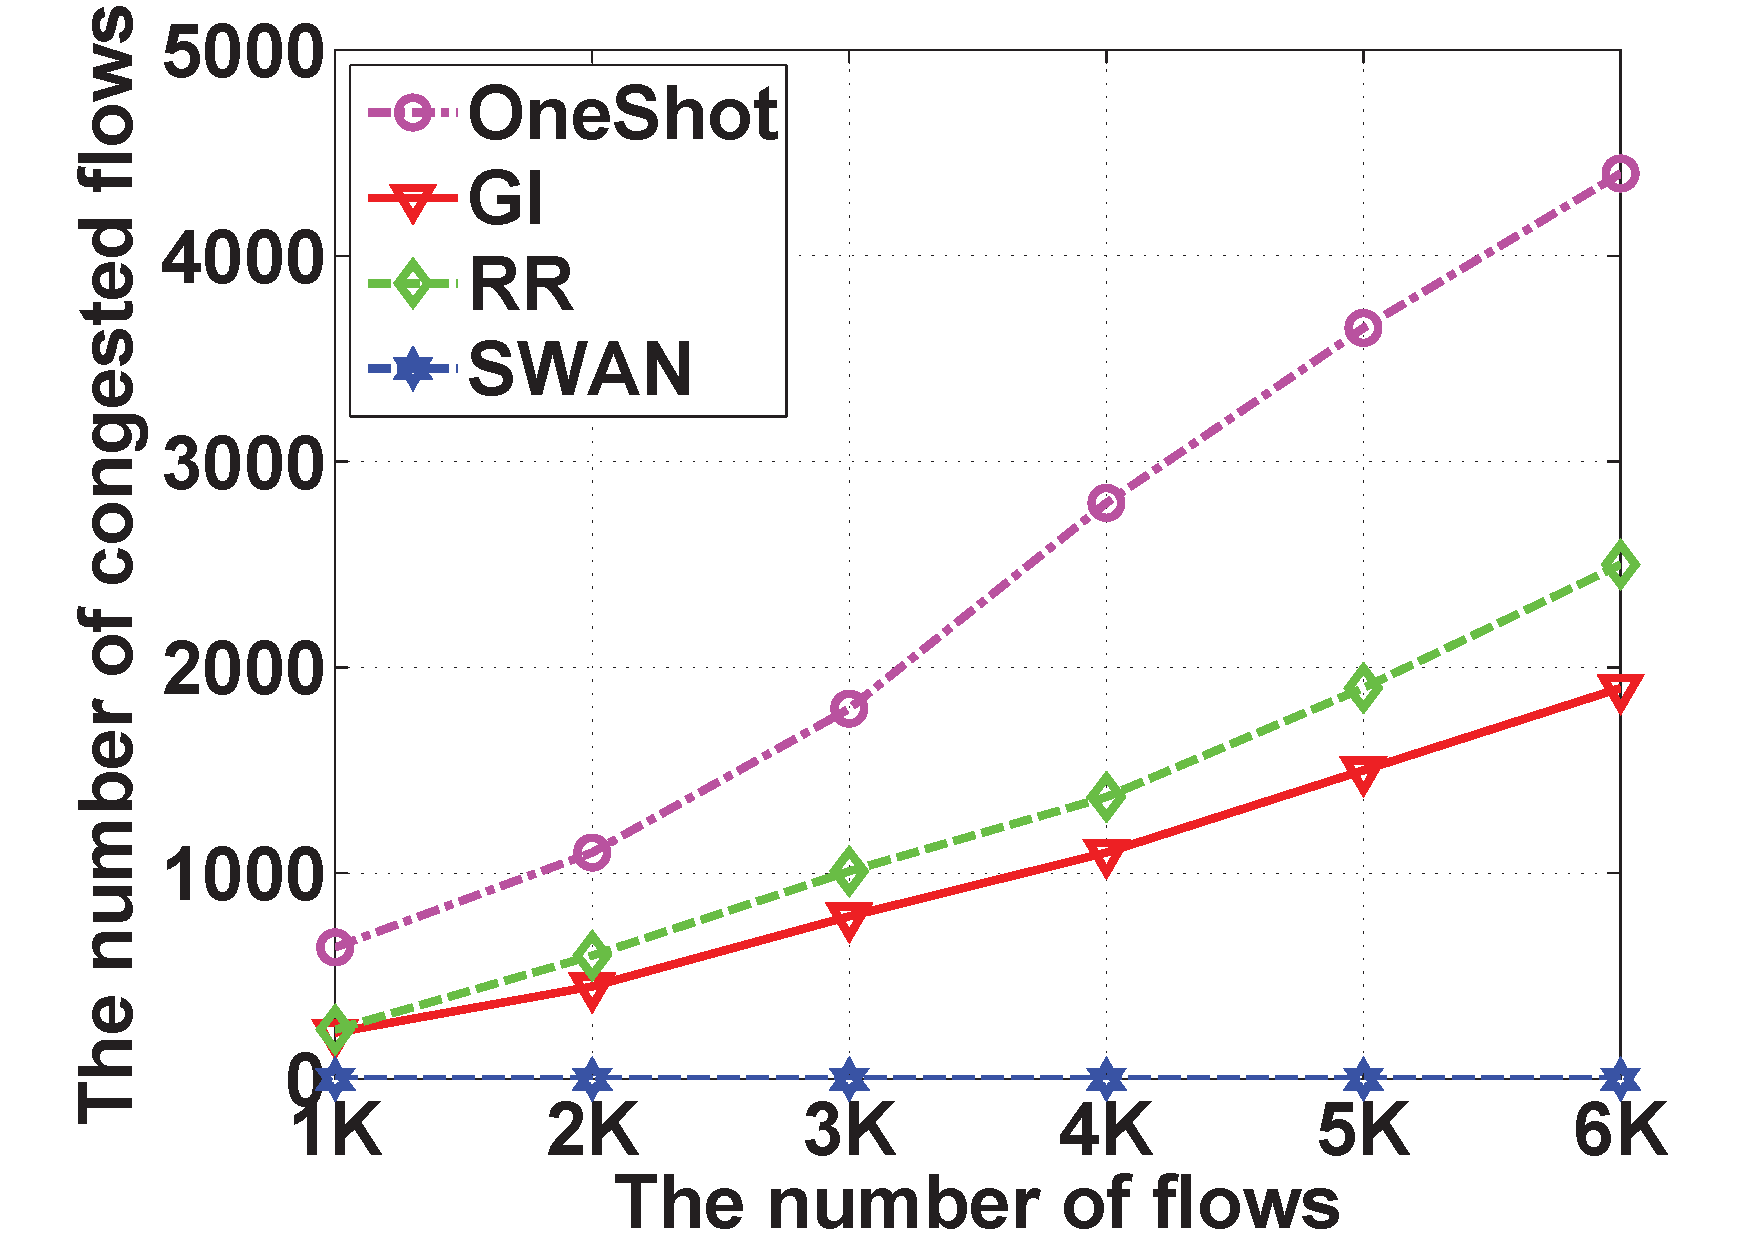
\includegraphics[width=1.6in]{Fig/RTWAN.pdf}}
\caption{The number of congested flows.}
\label{fig:RunningTime}
\end{minipage}
\vspace{-1em}
\end{figure*}

\subsection{tables}

\begin{table}[H]
\caption{Running time for finding congestion-free update plans}\label{Tab:RunningTime}
\centering
\begin{tabular}{|c|c|c|c|c|c|}
\hline
& 1K & 2K & 3K & 4K & 5K  \\
\hline
DCN & 0.73 min & 1.40 min & 2.10 min & 2.96 min &  4.12 min  \\
\hline
WAN & 0.60 min & 1.01 min & 1.57 min & 2.43 min & 3.12 min  \\
\hline
\end{tabular}
\begin{tabular}{l}
\\
write something to explain your table in here
\end{tabular}
\end{table}

%!TEX root = main.tex
\section{Conclusion}
\label{sec:conclusion}
In this paper, we list the basic component of an academic paper and show how they are organized using LaTex.

% remember \usepackage[cmex10]{amsmath}

% remember \usepackage{algorithmic} \usepackage{algorithm}


% remember  \usepackage[pdftex]{graphicx}  \usepackage[tight,footnotesize]{subfigure} \usepackage{tabularx}


%if figures don't align horizontally, try adjusting {0.x\textwidth} and [width=xinch]


\section{Acknowledgement}
We thank the anonymous reviewers for their helpful comments on draft of this paper.
The work is partly supported by XX project(maybe not).

\bibliography{cite}
\bibliographystyle{abbrv}

\appendices

\section{appendix section}

\end{document}